\section{Result and Analysis}
\subsection{Parameters}
\begin{table}[h]
    \centering
    \renewcommand{\arraystretch}{1.5} %
    \begin{tabular}{|c|c|}
        \hline
        \textbf{Parameters} & \textbf{Value} \\
        \hline
        \textbf{Total Datasets} & 7  \\
        \hline
        \textbf{Total images} & 446K  \\
        \hline
        \textbf{Trained images (real and fake)} & 203K , 203K \\
        \hline
        \textbf{Tested images (real and fake)} & 10K , 10K \\
        \hline
        \textbf{Validation (real and fake)} & 10K , 10K \\
        \hline
        \textbf{Balanced} &  True\\
        \hline
        \textbf{Epochs} &  10\\
        \hline
        \textbf{Batch Size} &  32\\
        \hline
        \textbf{Image Size} &  256 x 256\\
        \hline
        \textbf{Channels} &  3\\
        \hline
        \textbf{Patches} & 16 x 16\\
        \hline
        \textbf{Encoder Hidden Layers} & 12\\
        \hline
        \textbf{Encoder Layers Dimension} & 768\\
        \hline
        \textbf{MLP size} & 3072\\
        \hline
        \textbf{ Number of Attention Heads } & 12\\
        \hline
        \textbf{Loss Function} & Cross-Entropy Loss \\
        \hline
        \textbf{Normalization} & Layer Normalization \\
        \hline
        \textbf{Activation Function} & GeLU \\
        \hline
        \textbf{Dropout Rate } & 0.2  \\
        \hline
        \textbf{Pooling Strategy } & CLS Token \\
        \hline
    \end{tabular}
    \caption{Model Parameters}
    \label{tab:model-parameters}
\end{table}
\subsection{Work Completed}
\subsubsection{User Interface of Mobile application}
\begin{itemize}
    \item Registration of new user.
    \item User Login.
    \item Interactive home page.
    \item Upload Image Interface.
\end{itemize}
\subsubsection{User Interface of Web application}
\begin{itemize}
    \item Registration of new user.
    \item User Login.
    \item Interactive home page.
    \item Upload Image Interface.
\end{itemize}
\subsubsection{Backend}
\begin{itemize}
    \item API for registration of new user.
    \item API for user login.
    \item API to upload image.
\end{itemize}
\subsubsection{Machine Learning Model}
\begin{itemize}
    \item Real image data collected.
    \item Fake image data collected.
    \item Selection of ViT.
    \item Data cleaning and preprocessing.
    \item Extraction of attributes(parameters).
    \item Employing Embedding techniques.
    \item Visualization and interpretation.
    \item Preparation for model training.
\end{itemize}

\subsection{Work Remaining}
\begin{itemize}
    \item Integration of Backend.
    \item Model training.
    \item Model evaluation and validation.
\end{itemize}

\subsection{UI of Project}
We have used Flutter and Django to develop the mobile application in which we prepared a
UI with user authentication, login page and home page where we can upload images to be classified as fake and real.\\

\begin{figure}[ht]
    \centering
    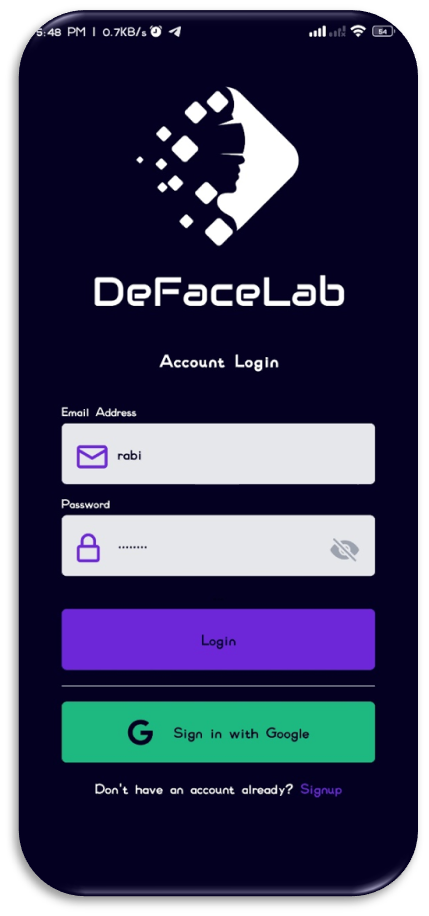
\includegraphics[ height =5in ]{img/loginv3.png}
    \caption{\textit{Login Page }}
\end{figure}

\begin{figure}[ht]
    \centering
    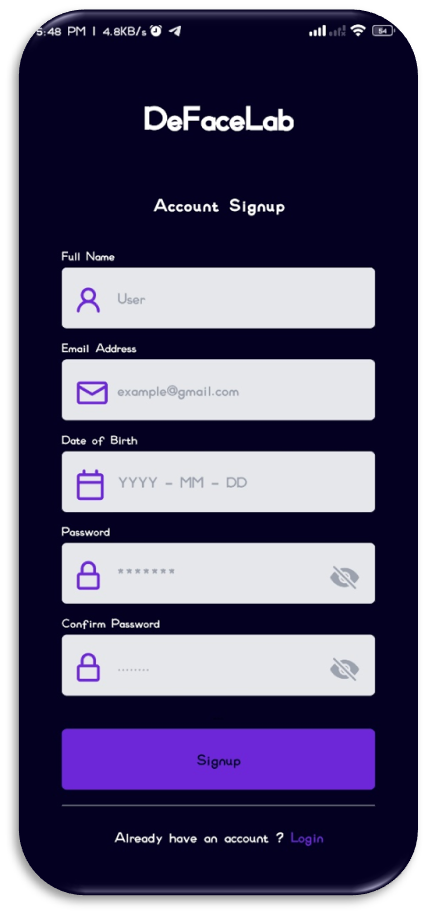
\includegraphics[height= 5in]{img/signup.png}
    \caption{\textit{Sign-up form}}
\end{figure}
\begin{figure}[ht]
    \centering
    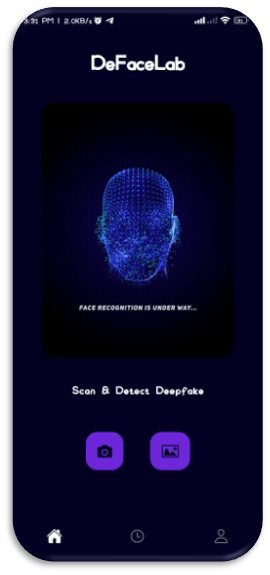
\includegraphics[height =5in ]{img/Homepage.png}
    \caption{\textit{Home Page}}
\end{figure}

\begin{figure}[ht]
    \centering
    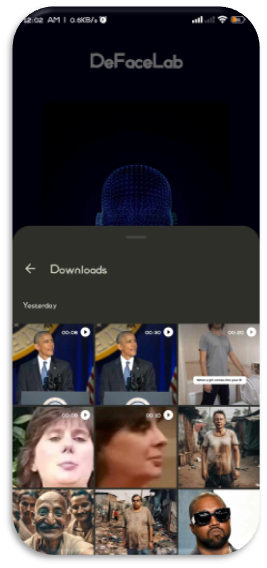
\includegraphics[height =5in ]{img/uploaderv3.png}
    \caption{\textit{Uploader}}
\end{figure}

\begin{figure}[ht]
    \centering
    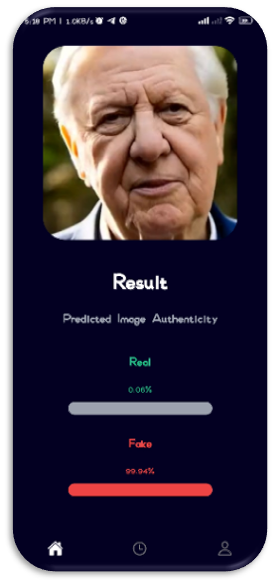
\includegraphics[height= 5in]{img/Results.png}
    \caption{\textit{Result}}
\end{figure}

\begin{figure}[ht]
    \centering
    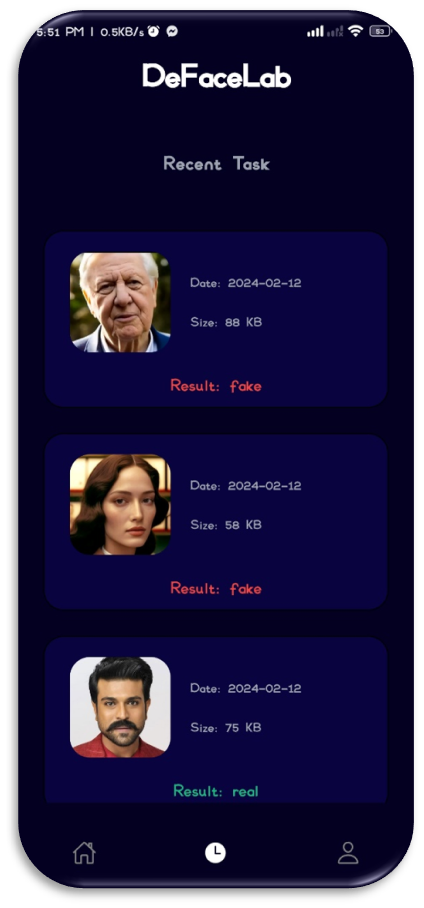
\includegraphics[height= 5in]{img/Historyv2.png}
    \caption{\textit{History page}}
\end{figure}


\begin{figure}[ht]
    \centering
    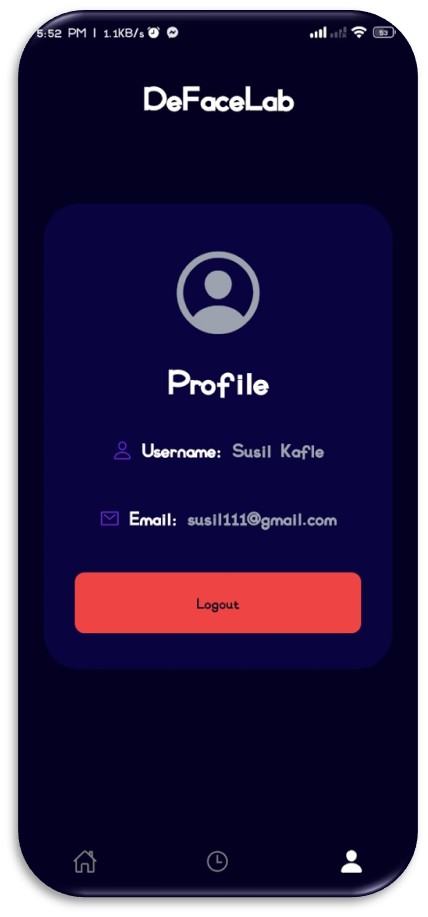
\includegraphics[height= 5in]{img/profilev2.png}
    \caption{\textit{Profile page}}
\end{figure}